%%%%%%%%%%%%%%%%%%%%%%%%%%%%%%%%%%%%%%%%%%%%%%%%%%%%%%%%%%%%%%%%%%%%%%
% How to use writeLaTeX: 
%
% You edit the source code here on the left, and the preview on the
% right shows you the result within a few seconds.
%
% Bookmark this page and share the URL with your co-authors. They can
% edit at the same time!
%
% You can upload figures, bibliographies, custom classes and
% styles using the files menu.
%
%%%%%%%%%%%%%%%%%%%%%%%%%%%%%%%%%%%%%%%%%%%%%%%%%%%%%%%%%%%%%%%%%%%%%%

\documentclass[12pt]{article}

\usepackage{sbc-template}

\usepackage{graphicx,url}

%\usepackage[brazil]{babel}   
\usepackage[utf8]{inputenc}  
\renewcommand{\refname}{Referências}
     
\sloppy

\title{Estudo preliminar: Uso da arquitetura deep learning de \textit{answer selection} no problema do \textit{code retrieval}}

\author{Marcelo de Rezende Martins\inst{1}, Marco Aurélio Gerosa\inst{2}}


\address{Instituto de Pesquisas Tecnológicas
  (IPT)\\
  São Paulo -- SP -- Brazil
\nextinstitute
  Northern Arizona University\\
  Flagstaff, AZ, US
  \email{rezende.martins@gmail.com, Marco.Gerosa@nau.edu}
}

\begin{document} 

\maketitle

\begin{abstract}
  This meta-paper describes the style to be used in articles and short papers
  for SBC conferences. For papers in English, you should add just an abstract
  while for the papers in Portuguese, we also ask for an abstract in
  Portuguese (``resumo''). In both cases, abstracts should not have more than
  10 lines and must be in the first page of the paper.
\end{abstract}
     
\begin{resumo} 
  O problema do \textit{code retrieval} consiste em dado uma questão e um conjunto de trechos de código-fonte, recuperar o código fonte que resolva a questão . Este artigo busca apresentar uma nova abordagem para este problema, fazendo uma aproximação com o problema de \textit{answer selection} em \emph{NLP}. Sob esta perspectiva, pretendemos avaliar, inicialmente, o desempenho da arquitetura bi-LSTM com CNN no problema do \textit{code retrieval}. 
\end{resumo}


\section{Introdução}

Segundo \cite{Allamanis-bimodal-source-code-natural-language:2015}, \textit{code retrieval} é um problema de recuperar informação, 
dado uma questão ou descrição em linguagem natural e um conjunto de possíveis trechos de código-fonte, o objetivo é recuperar o 
trecho de código-fonte que solucione a questão ou seja mais relevante de acordo com a descrição. Já segundo \cite{lai-etal-2018-review},
dado uma questão e um conjunto de possíveis respostas, \textit{answer selection} busca identificar qual resposta consegue responder a 
pergunta corretamente. Pela definição, é possível verificar as similaridades dos problemas. \cite{iyer-etal-2016-summarizing} em seu trabalho, utilizou LSTM com o mecanismo de atenção para solucionar
o problema de \textit{code retrieval}. Tanto LSTM quanto o mecanismo de atenção é comumente utilizado nos problemas de tradução e geração de texto. Para \cite{Knuth:1984:LP}, 
o código-fonte é uma forma de comunicação:

\textit{"Let us change our traditional attitude to the construction of programs: Instead of imagining that our
main task is to instruct a computer what to do, let us
concentrate rather on explaining to human beings what
we want a computer to do."}

E \cite{Allamanis:2018:SML} apresenta a hipótese da naturalidade do código-fonte:

\textit{"\textbf{The naturalness hypothesis}. Software is a form of human communication; soft-
ware corpora have similar statistical properties to natural language corpora; and these
properties can be exploited to build better software engineering tools."}

Considerando o código-fonte uma forma de comunicação, assim elencado por \cite{Knuth:1984:LP} e reforçado por \cite{Allamanis:2018:SML} em sua hipótese, uma possível abordagem para o problema 
do \textit{code retrieval}, é analisá-la sob a perspectiva do \textit{answer selection}. Porém, é necessário levar em consideração as peculiaridades do código-fonte ao abordar o problema sob esta perspectiva. 

Este presente artigo busca apresentar os resultados preliminares de um estudo sobre o uso de arquitetura deep learning de answer selection no problema do code retrieval.
Inicialmente, utilizaremos a arquitetura bi-LSTM com CNN proposta por Tan et al.. Além de propor uma nova arquitetura para este problema, iremos avaliar o modelo 
utilizando os dados de entrada da base StaQC, criada por Yao. Yao coletou milhares de pares de perguntas e trechos de código-fonte do StackOverFlow e a 
disponibilizou publicamente. Yao avaliou a base utilizando a arquitetura proposta por Srinivasan Iyer, que combina uma rede neural LSTM com o mecanismo 
de atenção (attention). Esta arquitetura utilizada por Iyer é comumente utilizada na geração de textos, que foi a proposta do trabalho de Iyer. Além de criar um modelo
para recuperar o trecho de código-fonte a partir de uma descrição em linguagem natural, o modelo proposto por Iyer foi utilizada para fazer o inverso, gerar uma descrição
a partir de um trecho de código-fonte. A nossa proposta inicial é apenas recuperar o trecho de código-fonte a partir de uma descrição.

Na seção método é apresentado a arquitetura utilizada e as adaptações necessárias feitas. Na seção resultados iniciais discute-se os resultados e os ajustes nos 
parâmetros para evitar overfitting. Próximos passos e trabalhos futuros é apresentado na seção conclusão.


\section{Método} \label{sec:metodo}

Conforme mencionado anteriormente, iremos abordar o problema do \textit{code retrieval} sob a perspectiva do \textit{answer selection}. Utilizaremos inicialmente
a arquitetura proposta por Tan et al., que utiliza a função de classificação \textit{pairwise} e uma arquitetura siamesa \cite{lai-etal-2018-review}. De acordo com 
\cite{lai-etal-2018-review}, o problema de \textit{answer selection} pode ser analisado sob duas formas: forma de aprendizado e arquitetura.

\subsection{Forma de aprendizado}

O problema de \textit{answer selection} consiste em encontrar a resposta mais relevante dado uma questão. Ele pode ser abordado como uma problema de classificação, onde
o objetivo é classificar com uma pontuação melhor as respostas mais relevantes de acordo com a questão.

Tan et al. utilizou o método \textit{pairwise}, no qual ele classifica as respostas corretas com uma pontuação maior que a pontuação das incorretas. Dado uma questão,
o método utiliza pares de candidatos de repostas e aprende a classificar qual resposta é mais relevante para a questão. Por exemplo, os dados de entrada de treinamento
são triplas (q\_i, c\_i+, c\_i-), onde q\_i é uma questão, c\_i+ é uma resposta correta, c\_i- é uma resposta incorreta obtida a partir da amostra completa dos dados. 


 
Descrição breve do problema e do método utilizado. Arquitetura siamês, utilizando representação distribuída de código-fonte e questão com uma camada bi-LSTM conectada a um filtro CNN. E por fim, utiliza uma camada de agregação max pooling e utilizando a funcao hinge loss de ranking.

\subsection{Arquitetura}

\subsubsection{Representação}
Os dados foram representados como sequência de tokens. Utilizamos uma representação distribuída word2vec. Diferente do \textit{answer selection} proposto por Tan et al. no qual ele cria apenas uma representação distribuída para a amostra inteira, nós geramos a representação distribuída para as questões e outra para os trechos do código-fonte.

A amostra e a visualização dos dados são apresentados nos resultados preliminares.






\section{Resultados preliminares}\label{sec:resultados-preliminares}

\subsection{Dados}

Para visualizar a representação distribuída, utilizamos o método t-SNE. A representação pode ser visualizada nas imagens abaixo:

\begin{figure}[h]
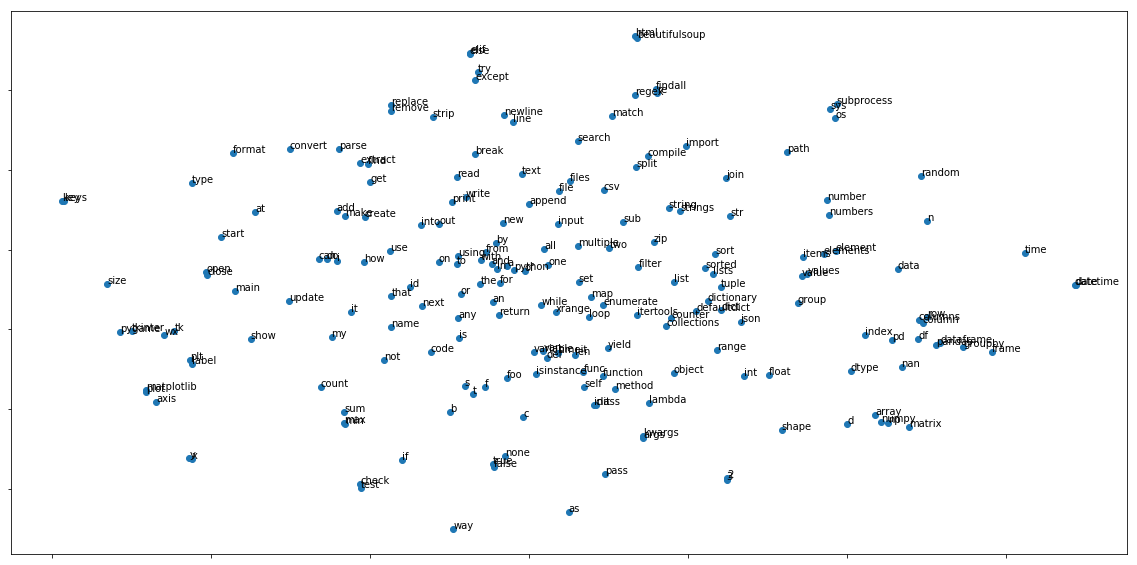
\includegraphics[width=14cm]{figures/tsne-question.png}
\caption{t-SNE para 200 palavras mais comuns das questões}
\label{fig:tsne-questao}
\end{figure}

\begin{figure}[h]
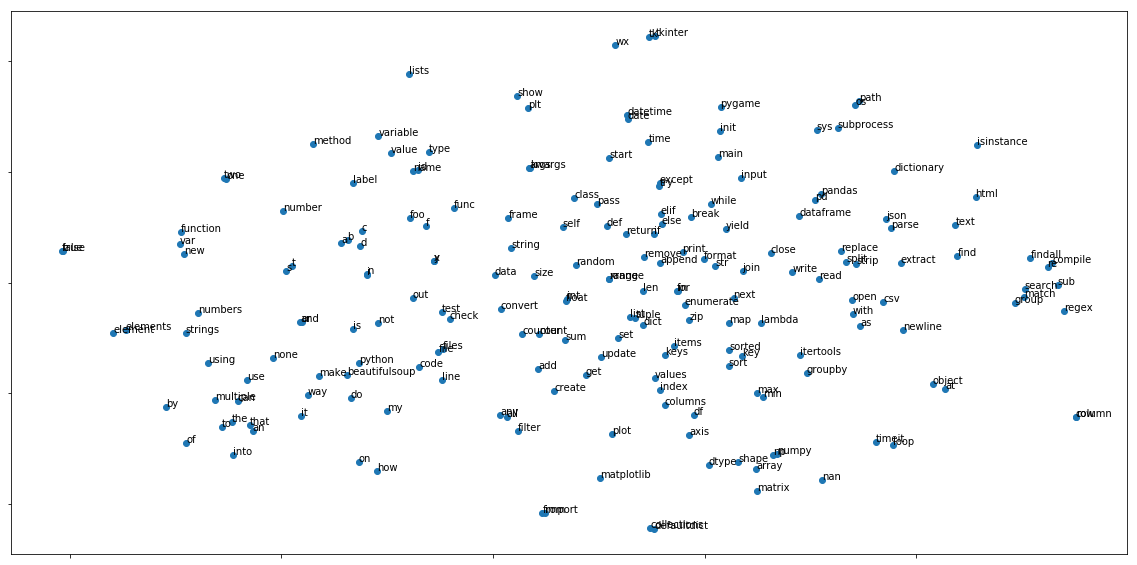
\includegraphics[width=14cm]{figures/tsne-code.png}
\caption{t-SNE para 200 palavras mais comuns dos trechos de código-fonte}
\label{fig:tsne-codigo}
\end{figure}

Adicionar os gráficos sobre a quantidade de palavras


\section{Conclusões}



\bibliographystyle{sbc}
\bibliography{sbc-template}


\end{document}
